% Options for packages loaded elsewhere
% Options for packages loaded elsewhere
\PassOptionsToPackage{unicode}{hyperref}
\PassOptionsToPackage{hyphens}{url}
\PassOptionsToPackage{dvipsnames,svgnames,x11names}{xcolor}
%
\documentclass[
  french,
  10pt,
  a4paper,
]{scrartcl}
\usepackage{xcolor}
\usepackage[top=1.7cm,bottom=1.7cm,left=1.6cm,right=1.6cm,headsep=0.35cm,footskip=0.75cm,includeheadfoot]{geometry}
\usepackage{amsmath,amssymb}
\setcounter{secnumdepth}{-\maxdimen} % remove section numbering
\usepackage{iftex}
\ifPDFTeX
  \usepackage[T1]{fontenc}
  \usepackage[utf8]{inputenc}
  \usepackage{textcomp} % provide euro and other symbols
\else % if luatex or xetex
  \usepackage{unicode-math} % this also loads fontspec
  \defaultfontfeatures{Scale=MatchLowercase}
  \defaultfontfeatures[\rmfamily]{Ligatures=TeX,Scale=1}
\fi
\usepackage{lmodern}
\ifPDFTeX\else
  % xetex/luatex font selection
\fi
% Use upquote if available, for straight quotes in verbatim environments
\IfFileExists{upquote.sty}{\usepackage{upquote}}{}
\IfFileExists{microtype.sty}{% use microtype if available
  \usepackage[]{microtype}
  \UseMicrotypeSet[protrusion]{basicmath} % disable protrusion for tt fonts
}{}
\makeatletter
\@ifundefined{KOMAClassName}{% if non-KOMA class
  \IfFileExists{parskip.sty}{%
    \usepackage{parskip}
  }{% else
    \setlength{\parindent}{0pt}
    \setlength{\parskip}{6pt plus 2pt minus 1pt}}
}{% if KOMA class
  \KOMAoptions{parskip=half}}
\makeatother
% Make \paragraph and \subparagraph free-standing
\makeatletter
\ifx\paragraph\undefined\else
  \let\oldparagraph\paragraph
  \renewcommand{\paragraph}{
    \@ifstar
      \xxxParagraphStar
      \xxxParagraphNoStar
  }
  \newcommand{\xxxParagraphStar}[1]{\oldparagraph*{#1}\mbox{}}
  \newcommand{\xxxParagraphNoStar}[1]{\oldparagraph{#1}\mbox{}}
\fi
\ifx\subparagraph\undefined\else
  \let\oldsubparagraph\subparagraph
  \renewcommand{\subparagraph}{
    \@ifstar
      \xxxSubParagraphStar
      \xxxSubParagraphNoStar
  }
  \newcommand{\xxxSubParagraphStar}[1]{\oldsubparagraph*{#1}\mbox{}}
  \newcommand{\xxxSubParagraphNoStar}[1]{\oldsubparagraph{#1}\mbox{}}
\fi
\makeatother

\usepackage{color}
\usepackage{fancyvrb}
\newcommand{\VerbBar}{|}
\newcommand{\VERB}{\Verb[commandchars=\\\{\}]}
\DefineVerbatimEnvironment{Highlighting}{Verbatim}{commandchars=\\\{\}}
% Add ',fontsize=\small' for more characters per line
\usepackage{framed}
\definecolor{shadecolor}{RGB}{241,243,245}
\newenvironment{Shaded}{\begin{snugshade}}{\end{snugshade}}
\newcommand{\AlertTok}[1]{\textcolor[rgb]{0.68,0.00,0.00}{#1}}
\newcommand{\AnnotationTok}[1]{\textcolor[rgb]{0.37,0.37,0.37}{#1}}
\newcommand{\AttributeTok}[1]{\textcolor[rgb]{0.40,0.45,0.13}{#1}}
\newcommand{\BaseNTok}[1]{\textcolor[rgb]{0.68,0.00,0.00}{#1}}
\newcommand{\BuiltInTok}[1]{\textcolor[rgb]{0.00,0.23,0.31}{#1}}
\newcommand{\CharTok}[1]{\textcolor[rgb]{0.13,0.47,0.30}{#1}}
\newcommand{\CommentTok}[1]{\textcolor[rgb]{0.37,0.37,0.37}{#1}}
\newcommand{\CommentVarTok}[1]{\textcolor[rgb]{0.37,0.37,0.37}{\textit{#1}}}
\newcommand{\ConstantTok}[1]{\textcolor[rgb]{0.56,0.35,0.01}{#1}}
\newcommand{\ControlFlowTok}[1]{\textcolor[rgb]{0.00,0.23,0.31}{\textbf{#1}}}
\newcommand{\DataTypeTok}[1]{\textcolor[rgb]{0.68,0.00,0.00}{#1}}
\newcommand{\DecValTok}[1]{\textcolor[rgb]{0.68,0.00,0.00}{#1}}
\newcommand{\DocumentationTok}[1]{\textcolor[rgb]{0.37,0.37,0.37}{\textit{#1}}}
\newcommand{\ErrorTok}[1]{\textcolor[rgb]{0.68,0.00,0.00}{#1}}
\newcommand{\ExtensionTok}[1]{\textcolor[rgb]{0.00,0.23,0.31}{#1}}
\newcommand{\FloatTok}[1]{\textcolor[rgb]{0.68,0.00,0.00}{#1}}
\newcommand{\FunctionTok}[1]{\textcolor[rgb]{0.28,0.35,0.67}{#1}}
\newcommand{\ImportTok}[1]{\textcolor[rgb]{0.00,0.46,0.62}{#1}}
\newcommand{\InformationTok}[1]{\textcolor[rgb]{0.37,0.37,0.37}{#1}}
\newcommand{\KeywordTok}[1]{\textcolor[rgb]{0.00,0.23,0.31}{\textbf{#1}}}
\newcommand{\NormalTok}[1]{\textcolor[rgb]{0.00,0.23,0.31}{#1}}
\newcommand{\OperatorTok}[1]{\textcolor[rgb]{0.37,0.37,0.37}{#1}}
\newcommand{\OtherTok}[1]{\textcolor[rgb]{0.00,0.23,0.31}{#1}}
\newcommand{\PreprocessorTok}[1]{\textcolor[rgb]{0.68,0.00,0.00}{#1}}
\newcommand{\RegionMarkerTok}[1]{\textcolor[rgb]{0.00,0.23,0.31}{#1}}
\newcommand{\SpecialCharTok}[1]{\textcolor[rgb]{0.37,0.37,0.37}{#1}}
\newcommand{\SpecialStringTok}[1]{\textcolor[rgb]{0.13,0.47,0.30}{#1}}
\newcommand{\StringTok}[1]{\textcolor[rgb]{0.13,0.47,0.30}{#1}}
\newcommand{\VariableTok}[1]{\textcolor[rgb]{0.07,0.07,0.07}{#1}}
\newcommand{\VerbatimStringTok}[1]{\textcolor[rgb]{0.13,0.47,0.30}{#1}}
\newcommand{\WarningTok}[1]{\textcolor[rgb]{0.37,0.37,0.37}{\textit{#1}}}

\usepackage{longtable,booktabs,array}
\newcounter{none} % for unnumbered tables
\usepackage{calc} % for calculating minipage widths
% Correct order of tables after \paragraph or \subparagraph
\usepackage{etoolbox}
\makeatletter
\patchcmd\longtable{\par}{\if@noskipsec\mbox{}\fi\par}{}{}
\makeatother
% Allow footnotes in longtable head/foot
\IfFileExists{footnotehyper.sty}{\usepackage{footnotehyper}}{\usepackage{footnote}}
\makesavenoteenv{longtable}
\usepackage{graphicx}
\makeatletter
\newsavebox\pandoc@box
\newcommand*\pandocbounded[1]{% scales image to fit in text height/width
  \sbox\pandoc@box{#1}%
  \Gscale@div\@tempa{\textheight}{\dimexpr\ht\pandoc@box+\dp\pandoc@box\relax}%
  \Gscale@div\@tempb{\linewidth}{\wd\pandoc@box}%
  \ifdim\@tempb\p@<\@tempa\p@\let\@tempa\@tempb\fi% select the smaller of both
  \ifdim\@tempa\p@<\p@\scalebox{\@tempa}{\usebox\pandoc@box}%
  \else\usebox{\pandoc@box}%
  \fi%
}
% Set default figure placement to htbp
\def\fps@figure{htbp}
\makeatother



\ifLuaTeX
\usepackage[bidi=basic,shorthands=off]{babel}
\else
\usepackage[bidi=default,shorthands=off]{babel}
\fi
\ifLuaTeX
  \usepackage{selnolig} % disable illegal ligatures
\fi


\setlength{\emergencystretch}{3em} % prevent overfull lines

\providecommand{\tightlist}{%
  \setlength{\itemsep}{0pt}\setlength{\parskip}{0pt}}



 


% Mise en page des PDF : LaTeX classique (Latin Modern), A4, compacte,
% entièrement lisible en noir et blanc. Chargé après le préambule de Quarto.
\usepackage{xcolor}
\definecolor{vertprofond}{HTML}{1C322D}
\definecolor{grisfilet}{HTML}{A1A1AA}

% Paragraphes sans alinéa, séparés par un petit espace.
\setlength{\parindent}{0pt}
\setlength{\parskip}{0.5ex plus 0.2ex minus 0.1ex}

% Titres resserrés, en vert profond (assez sombre pour l'impression N&B).
\setkomafont{disposition}{\normalfont\bfseries\color{vertprofond}}
\setkomafont{section}{\large}
\setkomafont{subsection}{\normalsize}
\setkomafont{subsubsection}{\normalsize\itshape}
\RedeclareSectionCommand[beforeskip=-1.6ex plus -0.4ex minus -0.2ex,
  afterskip=0.6ex plus 0.1ex]{section}
\RedeclareSectionCommand[beforeskip=-1.2ex plus -0.3ex minus -0.2ex,
  afterskip=0.4ex plus 0.1ex]{subsection}
\RedeclareSectionCommand[beforeskip=-1ex plus -0.2ex,
  afterskip=0.3ex]{subsubsection}

% Listes serrées.
\usepackage{enumitem}
\setlist{topsep=0.3ex, itemsep=0.15ex, parsep=0pt, partopsep=0pt}

% Figures et tableaux : peu d'espace autour, images plafonnées en hauteur
% pour qu'un schéma n'occupe jamais une demi-page.
\setlength{\textfloatsep}{1.2ex plus 0.4ex minus 0.4ex}
\setlength{\floatsep}{1ex plus 0.4ex minus 0.4ex}
\setlength{\intextsep}{1ex plus 0.4ex minus 0.4ex}
\setlength{\abovecaptionskip}{0.4ex}
\setlength{\belowcaptionskip}{0pt}
\setkomafont{caption}{\small\itshape}
\setkomafont{captionlabel}{\small\itshape}
\setkeys{Gin}{width=\linewidth, height=0.28\textheight, keepaspectratio}
\renewcommand{\arraystretch}{1.15}

% En-tête et pied de page : formation et chapitre en haut, titre et
% numéro de page en bas. Les valeurs viennent du partial title.tex.
\usepackage{lastpage}
\usepackage[headsepline=0.4pt, footsepline=0.4pt]{scrlayer-scrpage}
\clearpairofpagestyles
\setkomafont{pageheadfoot}{\footnotesize\color{vertprofond}}
\setkomafont{pagenumber}{}
\ihead{\vintageformation}
\ohead{\vintagechapitre}
\ifoot*{\vintagetitre}
\ofoot*{\thepage\,/\,\pageref*{LastPage}}
\pagestyle{scrheadings}

% Schémas TikZ : les styles communs suivent dans tikz-vintage.tex.
\usepackage{tikz}
% Styles TikZ communs aux schémas du site (PDF et HTML).
% Lisibles en noir et blanc : le contraste vient des niveaux de gris,
% des traits (plein, tirets, pointillés) et des étiquettes, jamais de la
% seule couleur. Le vert profond de la charte sert de couleur d'encre.
\usetikzlibrary{arrows.meta, positioning, calc, fit, backgrounds,
  shapes.geometric, shapes.symbols, patterns, decorations.pathreplacing}
\definecolor{vertprofond}{HTML}{1C322D}
\definecolor{grisclair}{HTML}{E4E4E7}
\definecolor{grismoyen}{HTML}{A1A1AA}
\tikzset{
  >={Stealth[length=2.2mm]},
  every picture/.style={color=vertprofond, line width=0.6pt},
  every node/.style={font=\small},
  % Équipements
  poste/.style={draw, rounded corners=1.5pt, fill=white,
    minimum width=1.4cm, minimum height=0.8cm, align=center},
  serveur/.style={poste, fill=grisclair, minimum height=1cm},
  routeur/.style={draw, circle, fill=grisclair, minimum size=1cm,
    align=center, font=\small\bfseries},
  commutateur/.style={draw, fill=grismoyen!40, minimum width=2.4cm,
    minimum height=0.6cm, align=center, font=\small\bfseries},
  parefeu/.style={draw, fill=white,
    postaction={pattern=bricks, pattern color=grismoyen},
    minimum width=1.2cm, minimum height=0.9cm, font=\small\bfseries},
  nuage/.style={draw, cloud, cloud puffs=10, aspect=2, fill=white,
    align=center},
  % Liaisons
  lien/.style={line width=0.9pt},
  trunk/.style={line width=2pt},
  sans fil/.style={dashed},
  % Échanges de messages (diagrammes de séquence)
  ligne de vie/.style={dashed, grismoyen},
  message/.style={->},
  diffusion/.style={->, dashed},
  reponse/.style={->, densely dotted},
  % Annotations
  etiquette/.style={font=\footnotesize, inner sep=1pt, fill=white},
  adresse/.style={font=\footnotesize\ttfamily, inner sep=1pt},
  zone/.style={draw, dashed, rounded corners=4pt, inner sep=6pt},
}
\makeatletter
\@ifpackageloaded{tcolorbox}{}{\usepackage[skins,breakable]{tcolorbox}}
\@ifpackageloaded{fontawesome5}{}{\usepackage{fontawesome5}}
\definecolor{quarto-callout-color}{HTML}{909090}
\definecolor{quarto-callout-note-color}{HTML}{0758E5}
\definecolor{quarto-callout-important-color}{HTML}{CC1914}
\definecolor{quarto-callout-warning-color}{HTML}{EB9113}
\definecolor{quarto-callout-tip-color}{HTML}{00A047}
\definecolor{quarto-callout-caution-color}{HTML}{FC5300}
\definecolor{quarto-callout-color-frame}{HTML}{acacac}
\definecolor{quarto-callout-note-color-frame}{HTML}{4582ec}
\definecolor{quarto-callout-important-color-frame}{HTML}{d9534f}
\definecolor{quarto-callout-warning-color-frame}{HTML}{f0ad4e}
\definecolor{quarto-callout-tip-color-frame}{HTML}{02b875}
\definecolor{quarto-callout-caution-color-frame}{HTML}{fd7e14}
\makeatother
\makeatletter
\@ifpackageloaded{caption}{}{\usepackage{caption}}
\AtBeginDocument{%
\ifdefined\contentsname
  \renewcommand*\contentsname{Table des matières}
\else
  \newcommand\contentsname{Table des matières}
\fi
\ifdefined\listfigurename
  \renewcommand*\listfigurename{Liste des Figures}
\else
  \newcommand\listfigurename{Liste des Figures}
\fi
\ifdefined\listtablename
  \renewcommand*\listtablename{Liste des Tables}
\else
  \newcommand\listtablename{Liste des Tables}
\fi
\ifdefined\figurename
  \renewcommand*\figurename{Figure}
\else
  \newcommand\figurename{Figure}
\fi
\ifdefined\tablename
  \renewcommand*\tablename{Table}
\else
  \newcommand\tablename{Table}
\fi
}
\@ifpackageloaded{float}{}{\usepackage{float}}
\floatstyle{ruled}
\@ifundefined{c@chapter}{\newfloat{codelisting}{h}{lop}}{\newfloat{codelisting}{h}{lop}[chapter]}
\floatname{codelisting}{Listing}
\newcommand*\listoflistings{\listof{codelisting}{Liste des Listings}}
\makeatother
\makeatletter
\makeatother
\makeatletter
\@ifpackageloaded{caption}{}{\usepackage{caption}}
\@ifpackageloaded{subcaption}{}{\usepackage{subcaption}}
\makeatother
\usepackage{bookmark}
\IfFileExists{xurl.sty}{\usepackage{xurl}}{} % add URL line breaks if available
\urlstyle{same}
% fallback for those not using the hyperref driver hyperxmp:
\makeatletter
\@ifundefined{xmpquote}{\newcommand{\xmpquote}[1]{#1}}{}
\makeatother
\hypersetup{
  pdftitle={TP2 (partie 1) --- Premiers postes : poste à poste{,} adresses IP et concentrateur},
  pdflang={fr},
  colorlinks=true,
  linkcolor={vertprofond},
  filecolor={Maroon},
  citecolor={Blue},
  urlcolor={vertprofond},
  pdfcreator={LaTeX via pandoc}}


\newcommand{\vintagetitre}{TP2 (partie 1) --- Premiers postes : poste à
poste, adresses IP et concentrateur}
\newcommand{\vintageformation}{BTS CIEL 1}
\newcommand{\vintagechapitre}{01 --- Introduction aux réseaux}
\title{TP2 (partie 1) --- Premiers postes : poste à poste, adresses IP
et concentrateur}
\author{}
\date{}
\begin{document}
\thispagestyle{plain.scrheadings}
{\footnotesize\color{vertprofond}\textsc{BTS CIEL 1}\enspace·\enspace 01
--- Introduction aux réseaux\hfill \textsc{tp}\enspace·\enspace 1 h
30\par}
\vspace{0.6ex}
{\LARGE\bfseries\color{vertprofond}TP2 (partie 1) --- Premiers postes :
poste à poste, adresses IP et concentrateur\par}
\vspace{0.5ex}
{\itshape Prendre en main Packet Tracer, relier deux postes en réseau
poste à poste, leur donner des adresses IP, tester avec ping, puis
observer le rôle d'un concentrateur (hub).\par}
\vspace{0.3ex}
{\color{vertprofond}\rule{\linewidth}{0.8pt}\par}
\vspace{0.8ex}


\emph{Plateforme : Cisco Packet Tracer (postes PC-PT, concentrateurs
Hub-PT).}

\subsection{Objectifs et prérequis}\label{objectifs-et-pruxe9requis}

Pour que deux ordinateurs s'échangent des données, il faut un câble, une
adresse pour chacun et un moyen de vérifier que tout fonctionne. Dans ce
TP, vous construisez cela pas à pas, dans le simulateur, avec deux
postes puis avec cinq postes.

Ce TP est la première partie de « Création et interconnexions des LAN ».
Au fil des trois parties, vous allez :

\begin{itemize}
\tightlist
\item
  choisir le matériel pour construire un réseau poste à poste (Peer to
  Peer, P2P) ;
\item
  comprendre l'adressage IP ;
\item
  paramétrer des hôtes sur un même réseau pour qu'ils puissent
  communiquer entre eux ;
\item
  comprendre le fonctionnement d'un concentrateur (hub).
\end{itemize}

Les parties suivantes traitent du commutateur, du routeur, de la
passerelle, du réseau sans fil et d'un cahier des charges : voir la
\href{../tp-creation-lan-2/index.qmd}{partie 2} et la
\href{../tp-creation-lan-3/index.qmd}{partie 3}.

Vous avez déjà utilisé Packet Tracer dans le
\href{../tp-reseau-domestique/index.qmd}{TP1 --- Réseau domestique} :
vous savez placer un équipement et le relier par un câble.

\subsection{Situation de départ}\label{situation-de-duxe9part}

Vous devez équiper une petite salle informatique. Avant de passer au
matériel réel, vous testez vos choix dans un simulateur. Vous commencez
par le réseau le plus simple, deux ordinateurs reliés l'un à l'autre.
Vous le faites ensuite grandir avec un concentrateur.

Résultat attendu en fin de séance : un réseau de cinq postes reliés à un
concentrateur, puis un second concentrateur avec deux postes de plus, où
chaque poste joint tous les autres.

\subsection{Matériel et
environnement}\label{matuxe9riel-et-environnement}

\begin{tcolorbox}[enhanced jigsaw, arc=.35mm, bottomrule=.15mm, bottomtitle=1mm, breakable, colback=white, colbacktitle=quarto-callout-tip-color!10!white, colframe=quarto-callout-tip-color-frame, coltitle=black, left=2mm, leftrule=.75mm, opacityback=0, opacitybacktitle=0.6, rightrule=.15mm, title=\textcolor{quarto-callout-tip-color}{\faLightbulb}\hspace{0.5em}{Support d'activité}, titlerule=0mm, toprule=.15mm, toptitle=1mm]

\begin{itemize}
\tightlist
\item
  Cisco Packet Tracer, suite bureautique
\item
  Internet
\end{itemize}

\end{tcolorbox}

Vous rédigerez un compte rendu numérique. Pensez aux captures d'écran
pour illustrer votre compte rendu. Sauvegardez votre travail
régulièrement ! Des modifications peuvent exister selon la version du
logiciel utilisée.

\begin{longtable}[]{@{}ll@{}}
\caption{Contenu de cette partie}\label{tbl-sections}\tabularnewline
\toprule\noalign{}
Section & Contenu \\
\midrule\noalign{}
\endfirsthead
\toprule\noalign{}
Section & Contenu \\
\midrule\noalign{}
\endhead
\bottomrule\noalign{}
\endlastfoot
1 & Prise en main du simulateur réseau \\
2 & Faire communiquer les postes \\
3 & Adressage des hôtes sur le réseau \\
4 & Matériel nécessaire pour un réseau P2P \\
5 & Création d'un réseau avec concentrateur (hub) \\
\end{longtable}

\subsection{Travail à réaliser}\label{travail-uxe0-ruxe9aliser}

\subsubsection{1 --- Prise en main du simulateur
réseau}\label{prise-en-main-du-simulateur-ruxe9seau}

\paragraph{Création d'un réseau
P2P}\label{cruxe9ation-dun-ruxe9seau-p2p}

Vous allez dans un premier temps créer un réseau Peer-to-Peer constitué
de deux ordinateurs. Lancez le logiciel « Cisco Packet Tracer ». Vous
devez obtenir la fenêtre ci-dessous.

\begin{figure}[htbp]

{\centering \pandocbounded{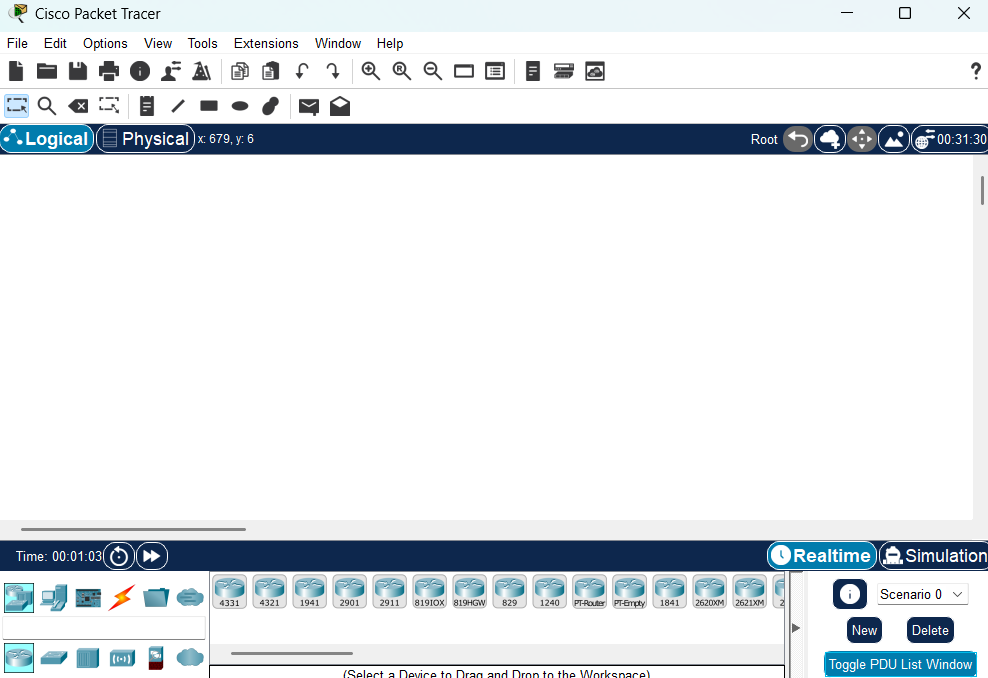
\includegraphics[keepaspectratio,alt={Capture d\textquotesingle écran de Packet Tracer au lancement : barre de menus et d\textquotesingle outils en haut, zone de travail logique vide au centre, palette des équipements et boutons Realtime et Simulation en bas.}]{img/fenetre-packet-tracer.png}}

}

\caption{La fenêtre de Packet Tracer au lancement.}

\end{figure}%

Pour ajouter un poste dans votre réseau, sélectionnez en bas à gauche de
l'écran la rubrique « Terminaux » (End Devices), cliquez sur l'icône «
Generic », puis cliquez dans la fenêtre pour y déposer un premier poste
: PC-PT PC0. Pour supprimer ce poste ou tout autre élément, cliquez sur
l'icône « Delete » à droite de l'écran, puis sélectionnez l'élément à
supprimer. Créez 2 postes « Generic », puis renommez-les comme
ci-dessous.

\begin{figure}[htbp]

{\centering \pandocbounded{
\includegraphics[keepaspectratio,alt={Capture d\textquotesingle écran de Packet Tracer : deux postes PC-PT, PC0 à gauche et PC1 à droite, non reliés.}]{img/deux-postes.png}}

}

\caption{Deux postes PC-PT nommés PC0 et PC1.}

\end{figure}%

Maintenant, il faut relier nos deux postes par un câble. Sélectionnez en
bas à gauche la rubrique « Connexions » (Connections), puis choisissez
un « câble droit » (Copper Straight-Through). Cliquez sur l'un et
l'autre poste pour mettre le câble (choisissez FastEthernet). Vous devez
obtenir le résultat suivant.

\begin{figure}[htbp]

{\centering \pandocbounded{
\includegraphics[keepaspectratio,alt={Capture d\textquotesingle écran de Packet Tracer : PC0 et PC1 reliés par un trait plein noir. Un triangle rouge marque chaque extrémité du câble.}]{img/cable-droit-rouge.png}}

}

\caption{Deux postes reliés par un câble droit : triangles rouges.}

\end{figure}%

La couleur rouge (aux extrémités du câble) indique qu'il y a un problème
dans l'installation de votre réseau. Il s'agit ici du fait qu'un câble
réseau droit a été utilisé. Pour relier des postes directement entre
eux, il faut utiliser un câble croisé.

Modifiez votre réseau : effacez le câble droit (touche « Suppr ») et
remplacez-le par un câble croisé (Copper Cross-Over).

\begin{figure}[htbp]

{\centering \pandocbounded{
\includegraphics[keepaspectratio,alt={Capture d\textquotesingle écran de Packet Tracer : PC0 et PC1 reliés par un trait pointillé noir. Un triangle vert marque chaque extrémité du câble.}]{img/cable-croise-vert.png}}

}

\caption{Deux postes reliés par un câble croisé : triangles verts.}

\end{figure}%

La couleur verte indique que la configuration matérielle est correcte et
que les postes ont maintenant la possibilité de communiquer entre eux.

\subsubsection{2 --- Faire communiquer les
postes}\label{faire-communiquer-les-postes}

Vous allez maintenant faire communiquer les deux postes d'un réseau P2P.
Lorsqu'un poste envoie des données à un matériel connecté au réseau, il
émet un message. Dans Packet Tracer, ce message s'appelle un
\textbf{PDU} (Protocol Data Unit, « unité de données de protocole ») :
c'est un bloc d'informations qui circule sur le support.

Cliquez sur l'icône « Add simple PDU » (à droite de l'écran). Cliquez
ensuite, dans l'ordre, sur le poste émetteur de l'information (PC0 par
exemple), puis sur le poste destinataire (PC1 par exemple).

\begin{figure}[htbp]

{\centering \pandocbounded{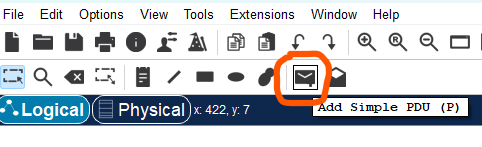
\includegraphics[keepaspectratio,alt={Capture d\textquotesingle écran de Packet Tracer : barre d\textquotesingle outils dont l\textquotesingle icône d\textquotesingle enveloppe fermée est entourée d\textquotesingle orange, avec l\textquotesingle info-bulle « Add Simple PDU (P) ».}]{img/icone-add-simple-pdu.png}}

}

\caption{L'icône « Add simple PDU » (enveloppe fermée) dans la barre
d'outils.}

\end{figure}%

Vous obtenez le message suivant en fenêtre.

\begin{figure}[htbp]

{\centering \pandocbounded{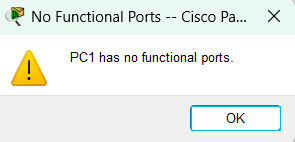
\includegraphics[keepaspectratio,alt={Capture d\textquotesingle écran d\textquotesingle une fenêtre « No Functional Ports -\/- Cisco Packet Tracer » indiquant « PC1 has no functional ports. » avec un bouton OK.}]{img/no-functional-ports.png}}

}

\caption{Message d'erreur : PC1 n'a aucun port fonctionnel.}

\end{figure}%

\subsubsection{3 --- Adressage des hôtes sur le
réseau}\label{adressage-des-huxf4tes-sur-le-ruxe9seau}

Lorsque vous envoyez un courrier à un destinataire, vous indiquez une
adresse sur l'enveloppe. Cette adresse comprend la rue, le code postal
et la ville. Lorsque La Poste achemine votre lettre, le code postal est
utilisé pour savoir dans quel département elle doit être remise. Ensuite
la ville est déterminée, et enfin la rue et le numéro de rue.

En matière de réseau, le fonctionnement est semblable. Un hôte du réseau
qui souhaite envoyer des données à un autre hôte doit indiquer l'adresse
de ce dernier sur le paquet qui est envoyé. Cette adresse s'appelle
l'\textbf{adresse IP} (IP pour Internet Protocol).

Une adresse IP correspond à un et un seul hôte sur un réseau. Elle
permet par conséquent d'identifier un hôte sur un réseau sans ambiguïté.

Vous allez définir des adresses IP pour chaque poste.

\begin{enumerate}
\def\labelenumi{\arabic{enumi}.}
\item
  Cliquez sur l'icône « Select » (en haut à droite), puis sur l'hôte «
  PC0 » pour ouvrir sa fenêtre de configuration.

  \begin{figure}[htbp]

  {\centering \pandocbounded{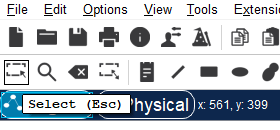
\includegraphics[keepaspectratio,alt={Capture d\textquotesingle écran de Packet Tracer : barre d\textquotesingle outils dont l\textquotesingle icône en forme de flèche pointillée porte l\textquotesingle info-bulle « Select (Esc) ».}]{img/icone-select.png}}

  }

  \caption{L'icône « Select » dans la barre d'outils.}

  \end{figure}%
\item
  Choisissez l'onglet « Desktop », puis « IP Configuration ».
\item
  Tapez l'adresse 192.168.0.1.
\item
  Cliquez dans la zone du masque de sous-réseau. Celui-ci est défini
  automatiquement : c'est le masque par défaut de la classe C,
  255.255.255.0.
\end{enumerate}

\begin{figure}[htbp]

{\centering \pandocbounded{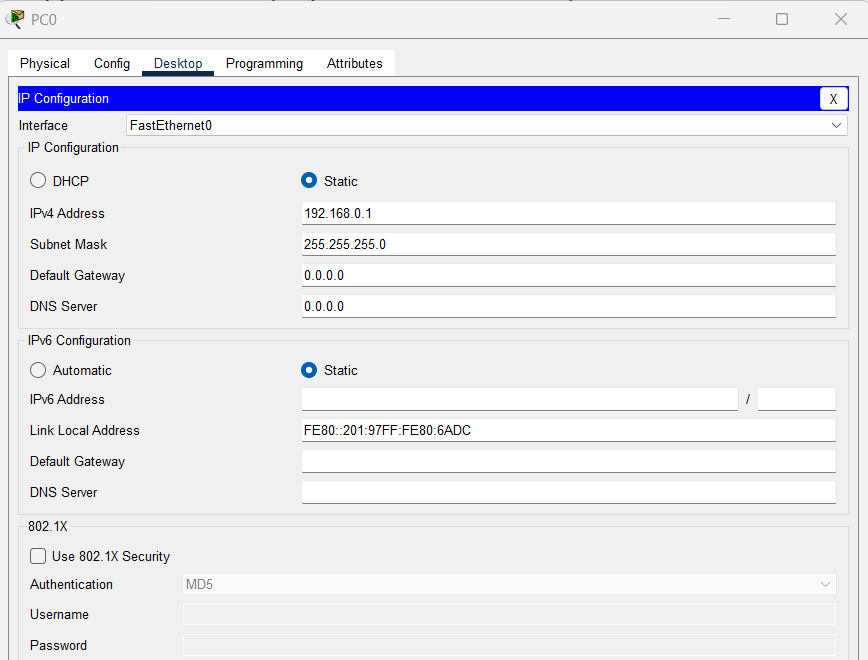
\includegraphics[keepaspectratio,alt={Capture d\textquotesingle écran de Packet Tracer : fenêtre de PC0, onglet Desktop, IP Configuration. L\textquotesingle option Static est cochée. IPv4 Address : 192.168.0.1. Subnet Mask : 255.255.255.0. Default Gateway : 0.0.0.0.}]{img/ip-configuration-pc0.png}}

}

\caption{Configuration IP de PC0 : adresse 192.168.0.1 et masque
255.255.255.0.}

\end{figure}%

\begin{enumerate}
\def\labelenumi{\arabic{enumi}.}
\setcounter{enumi}{4}
\tightlist
\item
  Faites de même pour l'autre poste, avec l'adresse IP 192.168.0.2.
\item
  Recommencez l'envoi d'un PDU entre les 2 postes : cette fois, la
  transmission s'est normalement déroulée.
\item
  Pour voir les détails de la transmission des données, cliquez sur «
  Toggle PDU List Window ».
\end{enumerate}

\begin{figure}[htbp]

{\centering \pandocbounded{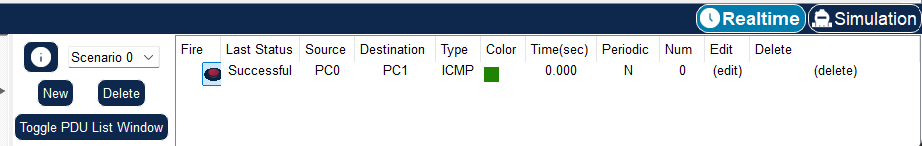
\includegraphics[keepaspectratio,alt={Capture d\textquotesingle écran de Packet Tracer : liste des PDU avec une ligne dont le statut est Successful, source PC0, destination PC1, type ICMP, couleur verte.}]{img/liste-pdu.png}}

}

\caption{La liste des PDU : envoi de PC0 vers PC1 réussi.}

\end{figure}%

Vous voyez que tout s'est bien déroulé, mais\ldots{} en temps réel.
C'est pourquoi vous n'avez rien vu : vous n'avez pas eu le temps de voir
quelque chose.

Pour ralentir le temps et observer l'envoi et la réception des PDU étape
par étape, passez en mode Simulation en cliquant sur l'icône en bas à
droite de l'écran.

\begin{figure}[htbp]

{\centering \pandocbounded{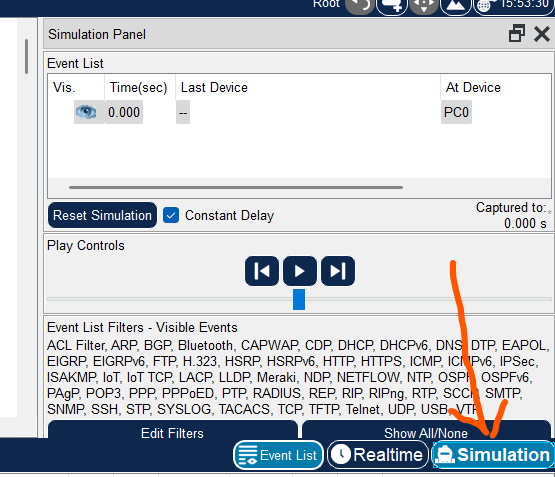
\includegraphics[keepaspectratio,alt={Capture d\textquotesingle écran de Packet Tracer : panneau de simulation avec la liste d\textquotesingle événements, les contrôles de lecture et la liste des filtres de protocoles. Une flèche orange désigne le bouton Simulation, en bas à droite.}]{img/mode-simulation.png}}

}

\caption{Le bouton « Simulation », en bas à droite de l'écran.}

\end{figure}%

Ensuite, cliquez plusieurs fois sur le bouton d'avance et observez ce
qui s'affiche dans la fenêtre de simulation. Ce bouton correspond à un
mode « pas à pas » : il faut cliquer à chaque fois pour voir les
échanges de données entre les postes.

\begin{figure}[htbp]

{\centering \pandocbounded{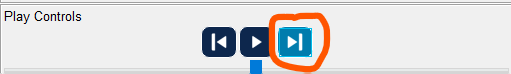
\includegraphics[keepaspectratio,alt={Capture d\textquotesingle écran des contrôles de lecture du panneau de simulation : le bouton d\textquotesingle avance pas à pas, à droite, est entouré d\textquotesingle orange.}]{img/bouton-avance.png}}

}

\caption{Le bouton d'avance pas à pas.}

\end{figure}%

\begin{figure}[htbp]

{\centering \pandocbounded{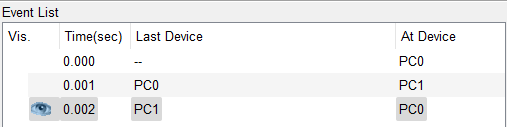
\includegraphics[keepaspectratio,alt={Capture d\textquotesingle écran de la liste d\textquotesingle événements en mode Simulation, avec trois lignes. À 0,000 s : appareil PC0. À 0,001 s : de PC0 vers PC1. À 0,002 s : de PC1 vers PC0.}]{img/event-list-ping.png}}

}

\caption{Exemple de liste d'événements : un PDU part de PC0 vers PC1,
puis revient de PC1 vers PC0.}

\end{figure}%

\begin{tcolorbox}[enhanced jigsaw, arc=.35mm, bottomrule=.15mm, bottomtitle=1mm, breakable, colback=white, colbacktitle=quarto-callout-note-color!10!white, colframe=quarto-callout-note-color-frame, coltitle=black, left=2mm, leftrule=.75mm, opacityback=0, opacitybacktitle=0.6, rightrule=.15mm, title=\textcolor{quarto-callout-note-color}{\faInfo}\hspace{0.5em}{Question 1}, titlerule=0mm, toprule=.15mm, toptitle=1mm]

Comment interprétez-vous ces informations ?

\end{tcolorbox}

\begin{tcolorbox}[enhanced jigsaw, arc=.35mm, bottomrule=.15mm, bottomtitle=1mm, breakable, colback=white, colbacktitle=quarto-callout-note-color!10!white, colframe=quarto-callout-note-color-frame, coltitle=black, left=2mm, leftrule=.75mm, opacityback=0, opacitybacktitle=0.6, rightrule=.15mm, title=\textcolor{quarto-callout-note-color}{\faInfo}\hspace{0.5em}{Question 2}, titlerule=0mm, toprule=.15mm, toptitle=1mm]

Cliquez sur l'enveloppe pour ouvrir le PDU. Dans quelle couche du modèle
OSI retrouve-t-on les adresses IP des postes ?

\end{tcolorbox}

\begin{tcolorbox}[enhanced jigsaw, arc=.35mm, bottomrule=.15mm, bottomtitle=1mm, breakable, colback=white, colbacktitle=quarto-callout-warning-color!10!white, colframe=quarto-callout-warning-color-frame, coltitle=black, left=2mm, leftrule=.75mm, opacityback=0, opacitybacktitle=0.6, rightrule=.15mm, title=\textcolor{quarto-callout-warning-color}{\faExclamationTriangle}\hspace{0.5em}{Filtre ICMP}, titlerule=0mm, toprule=.15mm, toptitle=1mm]

Cliquez sur « Edit Filters », puis cochez \textbf{uniquement} le
protocole ICMP. Nous ferons cela pour chaque simulation tout au long de
cette activité : nous ne visualiserons que l'échange des données au
niveau du protocole ICMP. Pensez donc, à chaque nouvelle construction de
réseau, à décocher l'ensemble des protocoles et à ne laisser que le
protocole ICMP.

\end{tcolorbox}

\paragraph{Requête d'écho ICMP}\label{requuxeate-duxe9cho-icmp}

Le \texttt{ping} (dont le nom s'inspire du son du sonar) est sans doute
l'un des outils d'administration réseau les plus connus et les plus
simples. Il permet, grâce à l'envoi de paquets ICMP (Internet Control
Message Protocol), de vérifier si une machine distante répond et, par
extension, si elle est bien accessible par le réseau.

Techniquement, \texttt{ping} envoie des paquets ICMP « Echo Request »
vers la machine cible et attend des réponses ICMP « Echo Reply ». Cette
communication permet de diagnostiquer la connectivité réseau et de
mesurer le temps de réponse (la latence). Chaque paquet ICMP est
transporté dans une trame sur le câble.

Sa mise en œuvre de base nécessite l'ouverture d'une fenêtre d'invite de
commande sous Windows, ou d'un terminal sous Linux ou Unix, comme la
plupart des outils de diagnostic réseau. La commande est :
\texttt{ping\ {[}adresse\ IP{]}} ou
\texttt{ping\ {[}nom\ d\textquotesingle{}hôte{]}}.

Le logiciel permet de simuler cette commande :

\begin{enumerate}
\def\labelenumi{\arabic{enumi}.}
\tightlist
\item
  Cliquez sur le poste « PC0 », choisissez l'onglet « Desktop », puis «
  Command Prompt ».
\item
  Tapez la commande suivante (invite de commandes d'un PC Packet
  Tracer), puis validez par la touche « Entrée » pour envoyer un ping
  vers l'autre poste :
\end{enumerate}

\begin{Shaded}
\begin{Highlighting}[]
\NormalTok{ping 192.168.0.2}
\end{Highlighting}
\end{Shaded}

\begin{enumerate}
\def\labelenumi{\arabic{enumi}.}
\setcounter{enumi}{2}
\tightlist
\item
  Réalisez la simulation en mode pas à pas.
\end{enumerate}

\begin{tcolorbox}[enhanced jigsaw, arc=.35mm, bottomrule=.15mm, bottomtitle=1mm, breakable, colback=white, colbacktitle=quarto-callout-note-color!10!white, colframe=quarto-callout-note-color-frame, coltitle=black, left=2mm, leftrule=.75mm, opacityback=0, opacitybacktitle=0.6, rightrule=.15mm, title=\textcolor{quarto-callout-note-color}{\faInfo}\hspace{0.5em}{Question 3}, titlerule=0mm, toprule=.15mm, toptitle=1mm]

Combien d'échanges y a-t-il eu entre les postes ? Quel est le temps
moyen d'échanges de données entre les postes ? En résumé, que permet de
voir un « ping » ?

\end{tcolorbox}

\begin{tcolorbox}[enhanced jigsaw, arc=.35mm, bottomrule=.15mm, bottomtitle=1mm, breakable, colback=white, colbacktitle=quarto-callout-warning-color!10!white, colframe=quarto-callout-warning-color-frame, coltitle=black, left=2mm, leftrule=.75mm, opacityback=0, opacitybacktitle=0.6, rightrule=.15mm, title=\textcolor{quarto-callout-warning-color}{\faExclamationTriangle}\hspace{0.5em}{Avertissement}, titlerule=0mm, toprule=.15mm, toptitle=1mm]

\textbf{ARRÊT : FAIRE VALIDER LE TRAVAIL PAR LE PROFESSEUR AVANT DE
POURSUIVRE}

\end{tcolorbox}

\subsubsection{4 --- Matériel nécessaire pour un réseau
P2P}\label{matuxe9riel-nuxe9cessaire-pour-un-ruxe9seau-p2p}

Le réseau Peer-to-Peer est le type de réseau nécessitant le moins de
matériel. Pour le mettre en place, il suffit d'utiliser :

\begin{itemize}
\tightlist
\item
  deux ordinateurs équipés chacun d'une carte réseau Ethernet ;
\item
  un câble à paires torsadées croisées muni de connecteurs RJ45 pour
  relier les cartes réseau.
\end{itemize}

Pour travailler avec ce réseau dans le logiciel tout en préservant votre
configuration, deux options s'offrent à vous :

\begin{enumerate}
\def\labelenumi{\arabic{enumi}.}
\tightlist
\item
  Enregistrez votre réseau via le menu « File » (Fichier), puis « Save »
  (Enregistrer). Par défaut, le fichier est sauvegardé dans le dossier
  du logiciel : enregistrez-le dans votre dossier personnel, ainsi que
  sur votre clé USB.
\item
  Créez un nouveau scénario en cliquant sur « New » (Nouveau) en bas de
  l'interface. Une fois le nouveau scénario créé, vous pouvez supprimer
  tous les équipements du réseau actuel pour en concevoir un nouveau.
\end{enumerate}

\subsubsection{5 --- Création d'un réseau avec concentrateur
(hub)}\label{cruxe9ation-dun-ruxe9seau-avec-concentrateur-hub}

Vous allez créer un réseau de cinq postes reliés par un concentrateur
(hub).

\begin{tcolorbox}[enhanced jigsaw, arc=.35mm, bottomrule=.15mm, bottomtitle=1mm, breakable, colback=white, colbacktitle=quarto-callout-note-color!10!white, colframe=quarto-callout-note-color-frame, coltitle=black, left=2mm, leftrule=.75mm, opacityback=0, opacitybacktitle=0.6, rightrule=.15mm, title=\textcolor{quarto-callout-note-color}{\faInfo}\hspace{0.5em}{Question 4}, titlerule=0mm, toprule=.15mm, toptitle=1mm]

Construisez le réseau conformément au schéma ci-dessous.

\end{tcolorbox}

\begin{figure}[htbp]

{\centering \pandocbounded{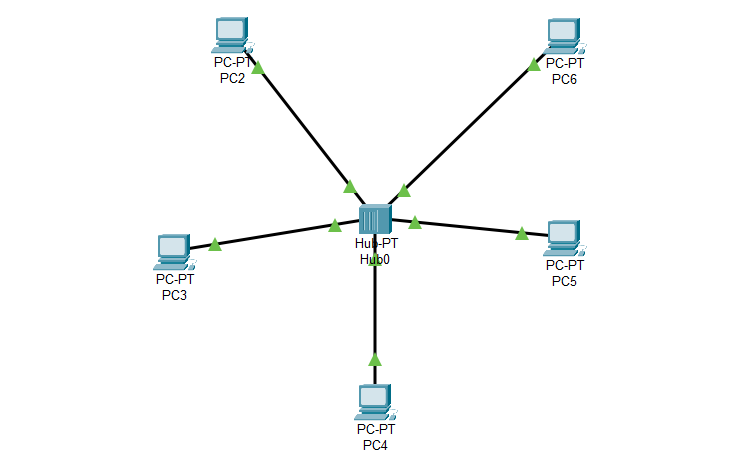
\includegraphics[keepaspectratio,alt={Schéma Packet Tracer : un concentrateur Hub-PT nommé Hub0 au centre. Cinq postes PC-PT sont reliés à lui par des traits pleins noirs : PC2 en haut à gauche, PC6 en haut à droite, PC3 à gauche, PC5 à droite et PC4 en bas. Tous les triangles sont verts.}]{img/reseau-hub.png}}

}

\caption{Cinq postes, PC2 à PC6, reliés à un concentrateur Hub0.}

\end{figure}%

\begin{tcolorbox}[enhanced jigsaw, arc=.35mm, bottomrule=.15mm, bottomtitle=1mm, breakable, colback=white, colbacktitle=quarto-callout-note-color!10!white, colframe=quarto-callout-note-color-frame, coltitle=black, left=2mm, leftrule=.75mm, opacityback=0, opacitybacktitle=0.6, rightrule=.15mm, title=\textcolor{quarto-callout-note-color}{\faInfo}\hspace{0.5em}{Question 5}, titlerule=0mm, toprule=.15mm, toptitle=1mm]

Quel type de câble a été utilisé pour relier les postes au concentrateur
? D'après la topologie physique des réseaux, quel est le type de réseau
que vous venez de construire ?

\end{tcolorbox}

\begin{tcolorbox}[enhanced jigsaw, arc=.35mm, bottomrule=.15mm, bottomtitle=1mm, breakable, colback=white, colbacktitle=quarto-callout-note-color!10!white, colframe=quarto-callout-note-color-frame, coltitle=black, left=2mm, leftrule=.75mm, opacityback=0, opacitybacktitle=0.6, rightrule=.15mm, title=\textcolor{quarto-callout-note-color}{\faInfo}\hspace{0.5em}{Question 6}, titlerule=0mm, toprule=.15mm, toptitle=1mm]

Configurez tous les postes en leur affectant une adresse IP statique de
classe C et un masque de sous-réseau (par défaut). Les postes font
partie d'un même réseau et peuvent donc communiquer ensemble.

\end{tcolorbox}

Pour vous aider, vous pouvez utiliser ces adresses, dans l'ordre des
numéros de poste, avec le masque 255.255.255.0 :

\begin{longtable}[]{@{}ll@{}}
\caption{Adresses proposées pour le réseau à
concentrateur}\label{tbl-adresses-hub}\tabularnewline
\toprule\noalign{}
Poste & Adresse IP \\
\midrule\noalign{}
\endfirsthead
\toprule\noalign{}
Poste & Adresse IP \\
\midrule\noalign{}
\endhead
\bottomrule\noalign{}
\endlastfoot
PC2 & 192.168.0.3 \\
PC3 & 192.168.0.4 \\
PC4 & 192.168.0.5 \\
PC5 & 192.168.0.6 \\
PC6 & 192.168.0.7 \\
\end{longtable}

Remarque : en plaçant le curseur sur un poste, vous visualiserez sa
configuration.

\begin{figure}[htbp]

{\centering \pandocbounded{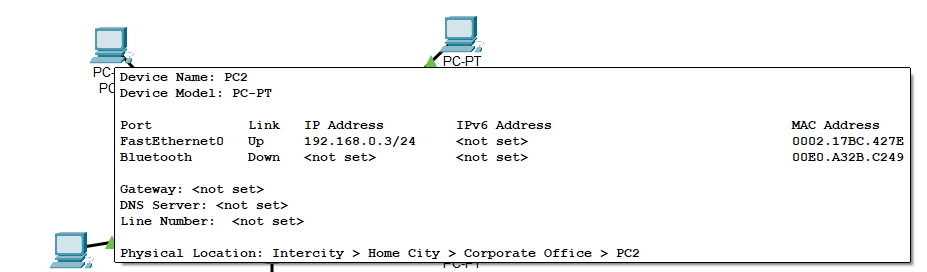
\includegraphics[keepaspectratio,alt={Capture d\textquotesingle écran de Packet Tracer : info-bulle du poste PC2, modèle PC-PT. Le port FastEthernet0 est Up, avec l\textquotesingle adresse IP 192.168.0.3/24 et l\textquotesingle adresse MAC 0002.17BC.427E. Le port Bluetooth est Down. Passerelle et serveur DNS non définis.}]{img/survol-pc2.png}}

}

\caption{Info-bulle du poste PC2 : port FastEthernet0 avec l'adresse
192.168.0.3/24.}

\end{figure}%

\begin{tcolorbox}[enhanced jigsaw, arc=.35mm, bottomrule=.15mm, bottomtitle=1mm, breakable, colback=white, colbacktitle=quarto-callout-note-color!10!white, colframe=quarto-callout-note-color-frame, coltitle=black, left=2mm, leftrule=.75mm, opacityback=0, opacitybacktitle=0.6, rightrule=.15mm, title=\textcolor{quarto-callout-note-color}{\faInfo}\hspace{0.5em}{Question 7}, titlerule=0mm, toprule=.15mm, toptitle=1mm]

En mode « Simulation », envoyez un PDU de PC2 vers PC4. Observez ce
qu'il se passe et visualisez le rôle du concentrateur. Envoyez un PDU de
PC2 vers PC5. Observez ce qu'il se passe et visualisez le rôle du
concentrateur. Quel est le rôle du concentrateur ? Comment
travaille-t-il ?

\end{tcolorbox}

\begin{tcolorbox}[enhanced jigsaw, arc=.35mm, bottomrule=.15mm, bottomtitle=1mm, breakable, colback=white, colbacktitle=quarto-callout-note-color!10!white, colframe=quarto-callout-note-color-frame, coltitle=black, left=2mm, leftrule=.75mm, opacityback=0, opacitybacktitle=0.6, rightrule=.15mm, title=\textcolor{quarto-callout-note-color}{\faInfo}\hspace{0.5em}{Question 8}, titlerule=0mm, toprule=.15mm, toptitle=1mm]

En mode « Simulation », envoyez deux PDU simultanément : de PC2 vers PC4
et de PC4 vers PC2. Observez ce qu'il se passe. Que s'est-il passé ?
Argumentez.

\end{tcolorbox}

En mode Simulation, vous pouvez avoir les informations d'un PDU (couche
OSI et trame) en double-cliquant sur l'enveloppe.

\begin{tcolorbox}[enhanced jigsaw, arc=.35mm, bottomrule=.15mm, bottomtitle=1mm, breakable, colback=white, colbacktitle=quarto-callout-note-color!10!white, colframe=quarto-callout-note-color-frame, coltitle=black, left=2mm, leftrule=.75mm, opacityback=0, opacitybacktitle=0.6, rightrule=.15mm, title=\textcolor{quarto-callout-note-color}{\faInfo}\hspace{0.5em}{Question 9}, titlerule=0mm, toprule=.15mm, toptitle=1mm]

Modifiez votre réseau de façon à avoir le réseau ci-dessous, avec deux
concentrateurs et deux autres postes configurés pour appartenir au même
réseau (par exemple 192.168.0.8 pour PC7 et 192.168.0.9 pour PC8).

\end{tcolorbox}

\begin{figure}[htbp]

{\centering \pandocbounded{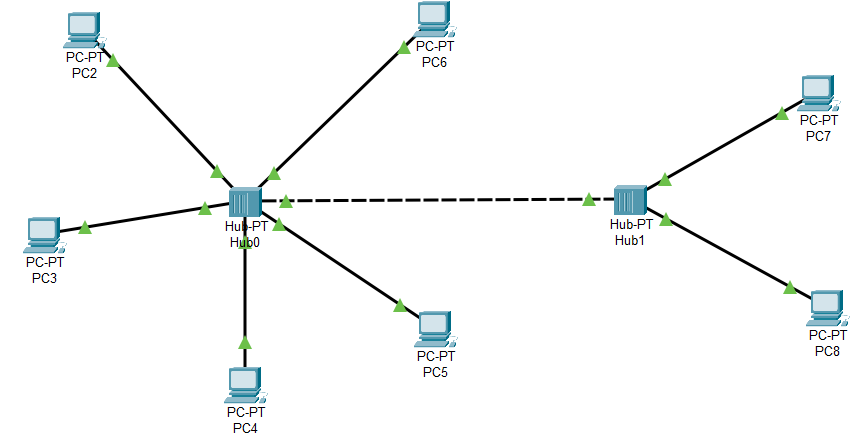
\includegraphics[keepaspectratio,alt={Schéma Packet Tracer : Hub0 relié aux postes PC2, PC3, PC4, PC5 et PC6 par des traits pleins noirs. Hub0 est relié à un second concentrateur, Hub1, par un trait pointillé noir. Hub1 est relié à PC7 et PC8 par des traits pleins. Tous les triangles sont verts.}]{img/reseau-deux-hubs.png}}

}

\caption{Deux concentrateurs reliés par un câble pointillé ; PC7 et PC8
sont reliés au second.}

\end{figure}%

\begin{tcolorbox}[enhanced jigsaw, arc=.35mm, bottomrule=.15mm, bottomtitle=1mm, breakable, colback=white, colbacktitle=quarto-callout-note-color!10!white, colframe=quarto-callout-note-color-frame, coltitle=black, left=2mm, leftrule=.75mm, opacityback=0, opacitybacktitle=0.6, rightrule=.15mm, title=\textcolor{quarto-callout-note-color}{\faInfo}\hspace{0.5em}{Question 10}, titlerule=0mm, toprule=.15mm, toptitle=1mm]

Quel type de câble utilise-t-on pour relier deux concentrateurs ?

\end{tcolorbox}

\begin{tcolorbox}[enhanced jigsaw, arc=.35mm, bottomrule=.15mm, bottomtitle=1mm, breakable, colback=white, colbacktitle=quarto-callout-note-color!10!white, colframe=quarto-callout-note-color-frame, coltitle=black, left=2mm, leftrule=.75mm, opacityback=0, opacitybacktitle=0.6, rightrule=.15mm, title=\textcolor{quarto-callout-note-color}{\faInfo}\hspace{0.5em}{Question 11}, titlerule=0mm, toprule=.15mm, toptitle=1mm]

Envoyez un PDU de PC2 vers PC7. Observez ce qu'il se passe. Que
pouvez-vous en conclure si le réseau compte un grand nombre d'hôtes
reliés à des concentrateurs ?

\end{tcolorbox}

\begin{tcolorbox}[enhanced jigsaw, arc=.35mm, bottomrule=.15mm, bottomtitle=1mm, breakable, colback=white, colbacktitle=quarto-callout-warning-color!10!white, colframe=quarto-callout-warning-color-frame, coltitle=black, left=2mm, leftrule=.75mm, opacityback=0, opacitybacktitle=0.6, rightrule=.15mm, title=\textcolor{quarto-callout-warning-color}{\faExclamationTriangle}\hspace{0.5em}{Avertissement}, titlerule=0mm, toprule=.15mm, toptitle=1mm]

\textbf{ARRÊT : FAIRE VALIDER LE TRAVAIL PAR LE PROFESSEUR AVANT DE
POURSUIVRE}

\end{tcolorbox}

\subsection{Vérification et compte
rendu}\label{vuxe9rification-et-compte-rendu}

Votre travail est réussi si vous pouvez constater les points suivants :

\begin{itemize}
\tightlist
\item
  deux postes reliés par un câble croisé affichent des triangles verts ;
\item
  \texttt{ping\ 192.168.0.2} lancé depuis PC0 reçoit des réponses ;
\item
  les cinq postes reliés à Hub0 se joignent tous entre eux ;
\item
  avec Hub1 et les postes PC7 et PC8, un PDU de PC2 atteint PC7.
\end{itemize}

Votre compte rendu contient :

\begin{itemize}
\tightlist
\item
  les réponses aux Questions 1 à 11 ;
\item
  une capture des deux postes reliés par le câble croisé (section 1) ;
\item
  une capture de la configuration IP de PC0 (section 3) ;
\item
  une capture de l'Event List d'un \texttt{ping} en mode Simulation,
  filtre ICMP seul (section 3) ;
\item
  une capture du réseau à un concentrateur (section 5) ;
\item
  une capture du réseau à deux concentrateurs pendant l'envoi de PC2
  vers PC7 (section 5).
\end{itemize}

Enregistrez votre maquette dans votre dossier personnel : les parties
suivantes la prolongent.

\subsection{Synthèse}\label{synthuxe8se}

\begin{tcolorbox}[enhanced jigsaw, arc=.35mm, bottomrule=.15mm, bottomtitle=1mm, breakable, colback=white, colbacktitle=quarto-callout-important-color!10!white, colframe=quarto-callout-important-color-frame, coltitle=black, left=2mm, leftrule=.75mm, opacityback=0, opacitybacktitle=0.6, rightrule=.15mm, title=\textcolor{quarto-callout-important-color}{\faExclamation}\hspace{0.5em}{Synthèse à compléter}, titlerule=0mm, toprule=.15mm, toptitle=1mm]

Recopiez et complétez ces phrases dans votre compte rendu.

\begin{enumerate}
\def\labelenumi{\arabic{enumi}.}
\tightlist
\item
  Pour relier directement deux postes, on utilise un câble
  \ldots\ldots\ldots\ldots{} .
\item
  Une adresse IP identifie un \ldots\ldots\ldots\ldots{} sur un réseau.
  Le masque par défaut d'une adresse de classe C est
  \ldots\ldots\ldots\ldots{} .
\item
  La commande \texttt{ping} envoie des paquets ICMP «
  \ldots\ldots\ldots\ldots{} » et attend des paquets ICMP «
  \ldots\ldots\ldots\ldots{} » .
\item
  Un concentrateur \ldots\ldots\ldots\ldots{} sur tous ses autres ports
  ce qu'il reçoit sur l'un de ses ports.
\item
  Quand beaucoup de postes sont reliés à des concentrateurs,
  \ldots\ldots\ldots\ldots{} .
\end{enumerate}

\end{tcolorbox}

Notez enfin, en deux ou trois lignes, la difficulté principale
rencontrée pendant ce TP et la manière dont vous l'avez résolue.

\subsection{Pour aller plus loin}\label{pour-aller-plus-loin}

Le \texttt{ping} repose sur le protocole ICMP, défini dans la RFC 792
(\emph{Internet Control Message Protocol}, IETF, 1981). Les adresses de
la plage 192.168.0.0/16, comme celles de ce TP, sont des adresses
privées : elles sont réservées aux réseaux locaux par la RFC 1918
(\emph{Address Allocation for Private Internets}, IETF, 1996).

Dans le simulateur, ajoutez un troisième poste à votre réseau P2P et
essayez de le relier directement à PC0 et à PC1 : de quel matériel
avez-vous besoin ? La partie 2 répond à cette question avec un
commutateur.




\end{document}
